\section{Security implementation in OSI levels}

\begin{figure}[h]
    \centering
    \includegraphics[page = 6,trim = 1cm 2.1cm 1cm 7cm, clip, width = 0.55\textwidth]{\slides}
\end{figure}

The main question is, “\textit{Which is the best OSI level to implement security?}” with many possibilities and answers. Typically, the “Presentation” layer is the only one in which security measures are not useful.

Unfortunately, \underline{there is not a single optimal level}. \textbf{The higher we go in the stack, the more specific our security functions can be}. For example, at the application level, it is possible to identify the user, commands, and data. Security functions are also independent of the underlying network, but if the functions are placed at the application level only, attacks at lower levels are possible (in particular, DoS attacks are available).

\textbf{The lower we go in the stack, the more quickly we can "expel" the intruders}, but the fewer data are available for the decision (e.g., only the MAC or IP addresses, no user identification, no commands).

In short, there is not an optimal level. You can decide whether to take one of these two risks or make a mixture by placing some security features at lower levels and then focus most of the security at the application level.


\subsection{DHCP (in)security}

When Layer 3 is reached, one of the first things activated is \textit{DHCP} because access to the network is given, and now the user needs to know the network parameters. DHCP is the protocol by which a device can ask to be assigned a valid network address. Unfortunately, the protocol is \textbf{non-authenticated} and a \textbf{broadcast protocol} that provides a response carrying \textit{IP address, netmask, default gateway, local nameserver,} and \textit{local DNS suffix}.

For this reason, the activation of a fake DHCP server is trivial because the DHCP request is a Layer 2 broadcast frame, and the only thing an attacker needs to do is to stay in the same broadcast domain as the victim and sniff the DHCP request.


Possible attacks from the fake DHCP are:

\begin{itemize}
    \item \textbf{Denial-of-service}:
          \begin{itemize}
              \item This can be done by providing a wrong network configuration.
          \end{itemize}

    \item \textbf{(Logical) Man-in-the-Middle (MITM)}:
          \begin{itemize}
              \item A valid IP address is provided to the victim, but it will be assigned a subnet with only the last two bits equal to zero. Therefore, only two addresses are valid: one of them is given to the user, and the other to the attacker as his default gateway. In that way, the attacked machine is isolated in a subnet of its own (logically, not physically). To communicate with all the nodes in the world, the victim has to send everything through the attacker.
              \item The replies could reach the original node without passing through the attacker. For this reason, it is possible to activate NAT, and it is possible to also intercept the replies.
          \end{itemize}

    \item \textbf{Malicious name-address translation}:
          \begin{itemize}
              \item The attacker declares himself as the local name server. Then, whenever the user needs to perform a name-to-address translation, the attacker will provide the wrong address. This is used, for example, for phishing and pharming.
          \end{itemize}
\end{itemize}

Various manufacturers have tried to provide some security improvement, such as switches (e.g., Cisco) that offer:

\begin{itemize}
    \item \textbf{DHCP Snooping}:
          \begin{itemize}
              \item Accepts only replies from "trusted ports."
          \end{itemize}

    \item \textbf{IP Guard}:
          \begin{itemize}
              \item Provides room only for IP addresses obtained from a valid DHCP server (but there is a limit on the number of recognized addresses).
          \end{itemize}
\end{itemize}

There is also RFC-3118 "Authentication for DHCP messages," which uses HMAC-MD5 to authenticate the messages, but it is rarely adopted because it is hardly configurable. Since HMAC is a symmetric protocol, it is needed to install a key on all the machines that need to use DHCP. This leads to the problem of key distribution. Furthermore, there is a problem of key management because if a key is captured, then it will be reusable, and since it is symmetric, any DHCP client could work as a DHCP server too.


\subsection{VPN}
\subsubsection{Security at Network Level (Layer 3)}

\begin{figure}[h]
    \centering
    \includegraphics[page = 10,trim = 2cm 2.2cm 2cm 10.5cm, clip, width = 0.55\textwidth]{\slides}
\end{figure}

Layer 3, which, given today's widespread use of the Internet, is predominantly IP, provides a crucial layer where meaningful security features can be implemented in a general sense. This is because it is the first layer that offers end-to-end connectivity. It allows for the creation of both \textbf{end-to-end protection} for Layer 3 homogeneous networks, such as IP networks, and \textbf{Virtual Private Networks (VPNs)}.

If it is possible to provide Layer 3 end-to-end protection, ensuring that data are secured as soon as they exit the server/client, it becomes irrelevant whether routers are properly managed or if the network being traversed is insecure. This is because the data are protected from the moment they exit the network interface until they reach the final network interface. Therefore, \ul{the only potential attacks are those originating from within the client/server}. Hence, security at Layer 3 allows us to disregard other attacks at the network level (except for Denial of Service - DoS).


\subsubsection{What is a VPN?}

\begin{figure}[h]
    \centering
    \includegraphics[page = 11,trim = 2cm 2.3cm 2cm 10cm, clip, width = 0.55\textwidth]{\slides}
\end{figure}


A \textit{Virtual Private Network} (VPN) is a technique, employing both hardware and/or software, that allows the creation of a private network while utilizing shared (or otherwise untrusted) channels and transmission devices. Instead of laying down their own cables and managing dedicated infrastructure, companies may prefer to establish a virtual segment of the network.

For instance, one could designate FIAT packets as "blue", allowing them to be exchanged only between blue endpoints. Similarly, packets from ENI could be labeled as "red" and permitted to be exchanged exclusively through red endpoints. While this conceptualization is beneficial, the devil lies in the details. Since it is impossible to visualize packets as blue or red, and the exact mechanism of their switching is uncertain, implementation details become crucial.

There are three techniques for creating a VPN:
\begin{itemize}
    \item \textbf{Private addressing}
    \item \textbf{Protected routing (IP tunnel)}
    \item \textbf{Cryptographic protection of network packets (secure IP tunnel)}
\end{itemize}


\paragraph*{VPN via Private Addresses}

In this basic VPN implementation, the networks included in the VPN use non-public addresses, making them unreachable from other networks (e.g., private IANA networks as listed in RFC-1918). Consequently, these networks are considered private, as they do not require authorization, and the packets in this case are not globally routable.

For example, a telecom provider wishing to share its infrastructure with various customers might allocate a distinct class of addresses to each customer. Access control lists (ACLs) on routers could then be implemented to ensure that packets are directed only to the allowed destinations.

However, this protection can be compromised under several circumstances:
\begin{itemize}
    \item \textbf{Guesses or discovers the addresses:} If the addresses are guessed or discovered, there is a risk of unauthorized access. If a class of addresses from another customer is found, an attacker could switch its own address to infiltrate that network.
    \item \textbf{Sniffing packets during transmission:} Since packets lack intrinsic protection, if network traffic can be sniffed, it may be possible to read the content of the packets.
    \item \textbf{Access to communication devices:} If someone gains access to the communication devices, they can read, change, or inject any type of packet.
\end{itemize}

There is minimal protection for packets, customers, and even for the infrastructure maintainer in this scenario. Consequently, the actual level of security is close to zero, despite the commercial availability of such services.


\paragraph{VPN via Tunnel}


This solution represents an improvement over the previous one. In this approach, routers encapsulate the entire Layer 3 packet as a payload within another packet, which can be \textbf{IP in IP}, \textbf{IP over MPLS}, or other techniques. Before encapsulation, border routers implement access control to the VPN via \textit{Access Control Lists} (\textbf{ACL}s). For instance, if a network belongs to the 10.1 address range, the destination can only be another network within the 10.1 range.

With this solution, providers gain protection against malicious end-users, as it prevents customers from changing the subnet to which they belong.
However, this protection can be circumvented by anyone managing a router or capable of sniffing packets during transmission. For instance, it does not provide protection to customers against attacks originating from within the geographical network (→ \ul{protection for providers but not for customers}).

If robust protection is desired, alternative techniques need to be considered.


\subparagraph{VPN via IP Tunnel}

\begin{figure}[h]
    \centering
    \includegraphics[page = 15,trim = 2cm 2.3cm 2cm 4cm, clip, width = 0.55\textwidth]{\slides}
    \caption{VPN via IP tunnel}
\end{figure}

Network 1 and Network 2 are depicted in the same color because they belong to the same subnet. When utilizing an IP tunnel, as the packets traverse from node A in subnet 1 to node B in subnet 2, they reach the border routers of subnet 1, which are responsible for encapsulation.

Router R1 identifies that B is in subnet 2, reachable through the border router R2. R1 then creates another packet that travels from R1 to R2, containing the original packet as its payload. The external IPv4 header of the tunnel is illustrated in the diagram. Upon receipt at router R2, the packet is decapsulated and forwarded to the final destination.

\textbf{Throughout transmission, the packet remains susceptible to being readable, manipulated, or injected}, signifying a lack of real security for the end user of the VPN.

The IP tunnel also presents a performance challenge: \textbf{fragmentation}. If the packet size equals the Maximum Transmission Unit (MTU), encapsulation will require fragmentation. In such instances, the maximum performance loss is 50\%, as two packets are generated instead of one. This impact is more pronounced for applications with large packets, typically non-interactive applications like file transfers. Consequently, this solution can also be a performance killer.


\paragraph{VPN via secure IP tunnel}

\begin{figure}[h]
    \centering
    \includegraphics[page = 17,trim = .4cm 4cm .5cm 5.5cm, clip, width = 0.55\textwidth]{\slides}
    \caption{VPN via secure IP tunnel}
    \label{fig:vpn-secure-ip}
\end{figure}

While the performance issue remains unresolved, the final solution offers enhanced security for end users. Prior to encapsulation, packets are protected with the following measures:
\begin{itemize}
    \item \textbf{MAC (Message Authentication Code):} Provides integrity and authentication.
    \item \textbf{Encryption:} Ensures confidentiality.
    \item \textbf{Numbering:} Guards against replay attacks.
\end{itemize}

No digital signature is employed due to its slowness, which would not align with the speed of current networks. If robust cryptographic algorithms are selected, the only viable attack is to disrupt communications (Denial of Service - DoS). This type of VPN is often referred to as \textbf{S-VPN} (\textit{Secure VPN}), representing the only VPN that can be considered secure (→ caution with VPNs promoted online).

In Figure \ref*{fig:vpn-secure-ip}, there is a router and a \textbf{TAP} (\textit{Tunnel Access Point}). Responsibilities are divided: the router oversees encapsulation/decapsulation, while the TAP is responsible for cryptographic protection. If this solution is implemented, and the TAP is managed by an external network provider, the security is compromised. Ideally, two separate devices should be in place: \ul{the client manages the TAP, and the ISP manages the router}.

\section{IPsec}

IPsec is the IETF architecture for Layer 3 security in IPv4/IPv6 designed to \textbf{create a Secure VPN (S-VPN) over untrusted networks} and \textbf{create end-to-end secure packet flows}. This is achieved through the definition of two specific packet types:

\begin{itemize}
    \item \textbf{AH (Authentication Header):}
          Provides integrity, authentication, and protection against replay attacks.
    \item \textbf{ESP (Encapsulating Security Payload):}
          Offers functions similar to AH, with the addition of payload confidentiality.
\end{itemize}

It is crucial to emphasize that \textbf{confidentiality can only be provided for the payload}; it is never possible to encrypt the header. Otherwise, intermediate systems would be unable to process the packets.

There is also a dedicated protocol for key exchange, named \textbf{IKE (Internet Key Exchange)}, to create and distribute keys in IP networks.

The IPsec security services include:

\begin{itemize}
    \item \textbf{Authentication of IP packets:}
          \begin{itemize}
              \item \textit{Data integrity}: The receiver can \textit{detect} if the packet has been manipulated. It is \underline{not} designed to prevent manipulation.
              \item \textit{Sender authentication}: A formal proof of the sender's identity. Note that this does not correspond to an IP address; IP addresses must not be trusted, as they can be completely fake (IP spoofing).
              \item \textit{(Partial) protection against "replay" attacks}: Challenges arise due to working at Layer 3, where packets can be lost or duplicated.
          \end{itemize}
    \item \textbf{Confidentiality of IP packets:}
          \begin{itemize}
              \item Data encryption (for the payload only).
          \end{itemize}
\end{itemize}



\begin{figure}[h]
    \centering
    \includegraphics[page = 20,trim = 2cm 3cm 2cm 10cm, clip, width = 0.55\textwidth]{\slides}
    \caption{IPsec Security Association (SA)}
    \label{fig:ipsec-sa}
\end{figure}

\subsection{Security Associations (SA)}

These security features are associated with the concept of \textbf{Security Association (SA)}, which is a \textbf{unidirectional logical connection between two IPsec systems}. Each SA is associated with different security services. To achieve full protection for a bidirectional packet flow between two nodes, \textbf{two SAs are needed} (one from A to B and one for the packets from B to A).

In theory, it is possible to have different security features and different algorithms for the two directions, but normally, even if there are two distinct SAs, the same kind of protection/algorithms are used.
Imagine that the sender (node A) is transmitting data (which may require confidentiality), but the response from B is a very simple thing (e.g., "received" or "bad") that does not need confidentiality. In this case, it is possible to avoid the encryption of the returning packet.

Security Associations are managed through two local databases, \textbf{which are not real databases}
(i.e., no implementation of servers like SQL, Oracle; it means that it is just \ul{a collection of data}):


\begin{itemize}
    \item \textbf{SPD (Security Policy Database):}
          \begin{itemize}
              \item It contains a list of security policies to apply to different packet flows.
              \item A-priori configured (e.g., manually) or connected to an automatic system (e.g., ISPS, which stands for Internet Security Policy System).
          \end{itemize}
    \item \textbf{SAD (SA Database):}
          \begin{itemize}
              \item It is a runtime database that contains the list of active SAs and their characteristics (e.g., algorithms, keys, parameters) to create protected traffic for that specific SA.
          \end{itemize}
\end{itemize}

\begin{figure}[h]
    \centering
    \includegraphics[page = 22,trim = 3cm 2.5cm 2cm 4.5cm, clip, width = 0.55\textwidth]{\slides}
    \caption{Local operations performed by a IPsec module when sending a packet}
\end{figure}

Suppose to be at a sending node within the TCP/IP stack. An IP packet has been created to be sent at L2, but on this node there's IPsec. When the packet is ready to be sent, the IPsec module starts working. The first question is: \textit{which policy should be applied for this packet?}

The answer is provided by the \textbf{SPD}. It can be \textit{"you should apply these security rules"} or \textit{"you don't need any kind of protection for this packet; go straight to L2"}.
If protection is needed and this is the first packet of this specific network flow, IPsec proceeds in creating a Security Association. Otherwise, there is already an existing SA, and it proceeds in reading the parameters associated with that SA by consulting the \textbf{SAD}. This will provide it with the algorithms and parameters to enrich the packet, and finally, the IP packet will be protected with IPsec and sent to L2 for the actual transmission.



\subsection{Transport mode IPsec}
\begin{figure}[h]
    \centering
    \includegraphics[page = 23,trim = 1cm 3cm 3cm 11cm, clip, width = 0.55\textwidth]{\slides}
    \caption{IPsec used for end-to-end security in transport mode}
\end{figure}

Transport Mode IPsec is used for \textbf{end-to-end security}, primarily employed by hosts rather than gateways (with the exception of traffic for the gateway itself, e.g., SNMP, ICMP). The original packet is split into two parts, and a new header is inserted between the IPv4 header and the TCP/UDP header. Thus, the IPv4 header will indicate that it is transporting IPsec (instead of TCP/UDP). Inside the IPsec header, there will be another field specifying the actual payload being transported.
\begin{itemize}
    \item \textbf{Pro:} It is computationally light.
    \item \textbf{Con:} No protection of header variable fields.
\end{itemize}


\subsection{Tunnel mode IPsec}
\begin{figure}[h]
    \centering
    \includegraphics[page = 24,trim = 1cm 3cm 2cm 9cm, clip, width = 0.55\textwidth]{\slides}
    \caption{IPsec used for end-to-end security in transport mode}
\end{figure}

Tunnel Mode IPsec is utilized to \textbf{create a VPN}, typically among \underline{gateways}. It is not created among routers; the correct term is gateway, which serves as a contact point between a network assumed to be secure and a network that is not secure. The gateway enhances protection by establishing the secure IPsec tunnel. It takes the original packet with the end-to-end header and encapsulates it inside a tunnel. This tunnel is initiated by the sending gateway and has the destination gateway protecting the network where the destination is located. The sending gateway applies IPsec to this IP in IP packet.

\begin{itemize}
    \item \textbf{Pro:} Complete protection of the packet, including header variable fields.
    \item \textbf{Con:} Computationally heavy.
\end{itemize}

Although not as common, IPsec in tunnel mode can also be used for end-to-end communication, even though it is typically adopted between border elements of larger networks. This setup is also known as a \textbf{site-to-site VPN} since the entities involved are typically entire networks.


\subsection{Authentication Header (AH)}
\begin{figure}[h]
    \centering
    \includegraphics[page = 26,trim = 1cm 6cm 1cm 5cm, clip, width = 0.55\textwidth]{\slides}
    \caption{IPsec AH header format according to RFC-4302}
\end{figure}

AH stands for \textbf{Authentication Header}. There have been three major versions of IPsec.

\subparagraph{Mechanism of the \textbf{first version} (RFC-1826):}
\begin{itemize}
    \item Data integrity and sender authentication
    \item Compulsory support of keyed-MD5 (RFC-1828)
    \item Optional support of keyed-SHA-1 (RFC-1852)
\end{itemize}

\subparagraph{Mechanism of the \textbf{second version} (RFC-2402):}
\begin{itemize}
    \item Data integrity, sender authentication, and (partial) protection from replay attacks
    \item HMAC-MD5-96
    \item HMAC-SHA-1-96
\end{itemize}

\subparagraph{Header format of the third version (RFC-4302)}
The format of the header added to the IPsec packet includes:
\begin{itemize}
    \item \texttt{Next header} field because this is a pseudo-protocol. In the IP header, it will indicate that it is transporting AH. Inside the AH, there is the real transporting packet field.
    \item \texttt{Length} parameter of 1 byte to describe the length of the packet.
    \item \texttt{Reserved} bytes for future uses.
    \item \texttt{Security Parameters Index (SPI)}: 32 bits to refer in a quick and easy way to all the parameters needed to verify in the packet.
    \item \texttt{Sequence number} to avoid replay attacks.
    \item \texttt{Integrity Check Value (ICV)}: Variable number of 4-byte words to provide authentication data (digest).
\end{itemize}



\begin{figure}[h]
    \centering
    \includegraphics[page = 27,trim = 1cm 2.1cm 1cm 2cm, clip, width = 0.90\textwidth]{\slides}
    \caption{The processing of a received IPsec packet}
    \label{fig:IPsec-receiving-packet}
\end{figure}

\paragraph{Receiving IPsec packet}
As shown in Figure \ref*{fig:IPsec-receiving-packet}, when an IPsec packet is received, it is protected with AH. The process begins with the \textbf{extraction} of the \texttt{AH}, and from it, the  \texttt{ICV} is extracted — the \texttt{received authentication value} (the digest computed by the sender).
Subsequently, the received packet undergoes \textbf{normalization}, which involves putting the packet in the same condition as it was at the sender to compute the same kind of hash.

Once the \texttt{normalized IP packet} is available, it is necessary to \textbf{compute the authentication value (ICV)}. For this purpose, the \textit{Security Parameter Index (SPI)} is used inside the \textit{Database of the Security Association (SAD)}. It serves as a pointer indicating the algorithm and parameters to be used. These parameters are employed to compute the authentication value, and then it is checked whether the two values (the one computed and the one received from the sender) are the same.

If the two values are equal, then the sender is authenticated, and the packet is integral. However, if the two values are not equal, there could be a fake sender and/or manipulated packet.

An authentic sender is identified in the previous picture, but there is no explicit mention of where the sender is authenticated. So, who is the sender authenticated here? The answer lies in the fact that a specific entry in the Security Association Database (SAD) is being utilized. This entry is negotiated with a specific node. For this reason, authentication is implicit in the process. The actual authentication comes into play when we create the Security Association: this is the point at which the sender must prove its identity. The Security Association (SA) ensures this form of authentication through the use of the correct algorithm/parameters.


\paragraph{HMAC-SHA1-96}
The key digest is based on HMAC, which includes an additional parameter '96' at the end. The HMAC-SHA1-96 is generated in the following way:

\begin{enumerate}
    \item Given $M$, normalize it to generate $M'$.
    \item Pad $M'$ to a multiple of 160 bits (by adding 0x00 bytes) to generate $M'p$.
    \item Compute the authentication base: $B = \texttt{HMAC-SHA1}(K, M'p)$ (where $K$ is the key agreed upon with the sender).
    \item $\text{ICV} = $ \textbf{the leftmost 96 bits of $B$}.
\end{enumerate}

Although we mentioned that a longer digest is needed to avoid various types of attacks, the decision to use only 96 bits may seem reckless. The reason behind this is a conflict of interest between security and network managers. Network managers prefer a header with a \textbf{fixed size}. If different algorithms are used for the digest, they may produce digests of varying lengths, posing a problem for router manufacturers dealing with variable-size headers. This approach might make it nearly impossible to process the header, resulting in lower resistance to replay attacks. In IPsec version 3, this aspect is further addressed.

\subsection{Encapsulating Security Payload (ESP)}
If confidentiality is desired, \textit{Encapsulating Security Payload} (\textit{ESP}) is required.
The first version (RFC-1827) provided only confidentiality. The basic mechanism operates on DES-CBC (RFC-1829), but other mechanisms are also possible. The second version also provided authentication, but not for the IP header, so the coverage is not equivalent to that of AH. The advantage is that the packet dimension is reduced, and one Security Association (SA) is saved.

\textbf{REMINDER:} IPsec is an architecture that is implemented with two kinds of packets: AH or ESP, \underline{and they may be used simultaneously}.

\paragraph*{}
ESP can be used in transport mode and tunnel mode as well.

\vspace*{5mm}
\noindent
\begin{minipage}{0.5\textwidth}
    \centering
    \includegraphics[page = 30,trim = 2cm 3cm 2cm 9cm, clip, width = \linewidth]{\slides}
\end{minipage}
\hspace{0.05\textwidth}
\begin{minipage}{0.4\textwidth}
    \paragraph{ESP in transport mode}
    If used in transport mode, ESP is inserted between the header and the payload. After a brief clear part, all the subsequent content will be encrypted, up to a \textbf{trailer} that concludes it.
    \begin{itemize}
        \item \textbf{Pro:} The payload is hidden, including information needed for Quality of Service (QoS), filtering, or intrusion detection.
        \item \textbf{Con:} The header remains in clear.
    \end{itemize}
\end{minipage}


\vspace*{5mm}
\noindent
\begin{minipage}{0.5\textwidth}
    \centering
    \includegraphics[page = 31,trim = 1cm 2.3cm 1cm 8cm, clip, width = \linewidth]{\slides}
\end{minipage}
\hspace{0.05\textwidth}
\begin{minipage}{0.4\textwidth}
    \paragraph{ESP in tunnel mode}
    If used in tunnel mode, the tunnel is first created, and then protection is applied to the tunnel payload. In this case, everything from the original packet is encrypted, including the end-to-end header.
\end{minipage}



\subsection{IPsec implementation details}

Since there are many algorithms that can be used, RFC-4308 defines two crypto-suites that anybody should implement for interoperability:

\begin{itemize}
    \item \textbf{VPN-A:} Uses ESP with 3DES-CBC and HMAC-SHA1-96. This is a legacy VPN for compatibility with old systems.
    \item \textbf{VPN-B:} Uses ESP with AES-128-CBC and AES-XCBC-MAC-96. This is the one used nowadays.
\end{itemize}

It is also possible to use \textbf{NULL algorithms} for ESP. You can specify \texttt{NULL} for one of the two parts: authentication or privacy, but not simultaneously. This allows for some kind of \textit{'protection against performance'} trade-off. Regarding the sequence number, it provides partial protection against replay attacks and works on a minimum window of 32 packets (64 suggested).


\subsection{IPsec Replay (partial) Protection}

When the sender is transmitting packets sequentially, they are numbered. However, since the network uses IP, these packets can be lost, duplicated, or arrive out-of-order, posing significant challenges. For instance, if the receiver has received packets 0-1-2 and then 4, can it declare that packet 3 was canceled by an attacker? The answer is uncertain due to the possibility of packet loss. Similarly, when the receiver has already received packet 53 and then receives packet 3, can it confidently claim that packet 3 is duplicated? No, as it could be an out-of-order packet.

To determine if a packet preceding the last received one is a duplicate, the only viable method is to maintain a list of received packets and check if the packet has already been received or not. However, maintaining a list of all received packets is impractical due to the potentially large number.

\begin{wrapfigure}{r}{0.50\textwidth}
    \centering
    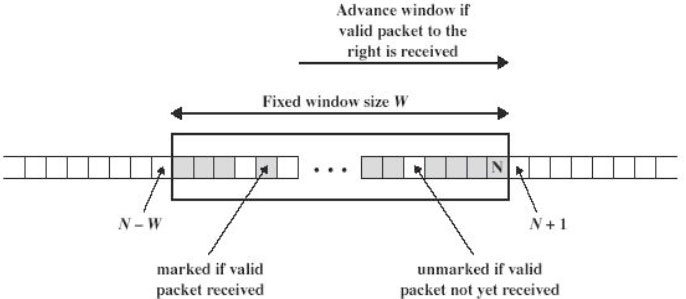
\includegraphics[width = 0.50\textwidth]{./chapter6/IPsec_replay_protection.png}
\end{wrapfigure}

Hence, a sliding window is employed, consisting of a \textbf{fixed window of size W}. In this window, received packets are marked, while unmarked packets remain unreceived. When an old packet is received, it is accepted if it belongs to an unreceived slot (indicating an out-of-order packet) and discarded if it was already received (indicating duplication from the network or an attacker).


If an old packet (outside the window) is received, there is no way to check its validity. This poses a significant risk because accepting it could result in a replay attack, while discarding it could lead to communication issues. If the protected traffic is \underline{TCP}, accepting an old packet is \underline{less risky}, as it will be discarded at the upper level if already received. However, for \underline{UDP} packets, \underline{accepting old packets is not allowed}, and the sender is usually requested to resend with a fresher sequence number.

The window progresses: when all packets up to 20 are received and packet 21 arrives, the window shifts one packet to the right. \textbf{Whenever a new packet with a sequence number greater than the current one is received, the window slides}. \textbf{Waiting for unreceived} packets is \textbf{not feasible}, as they could be lost (and IP does not handle retransmission).

\subsection{IPsec v3}

IPsec v3 changes the paradigm by providing equal support to the two headers. In fact, ESP is mandatory, and AH is optional. This means that it is possible to find implementations of IPsec that do not support AH, i.e., integrity and authentication for the payload only, not for the header. IPsec v3 has also added support for single-source multicast.

Moreover, since IPsec has been mainly used to create site-to-site VPNs, which involve channels with a lot of traffic, to avoid overflow of the sequence numbers, IPsec v3 has introduced \textbf{ESN} (Extended Sequence Number). ESN consists of 64 bits, even though inside packets there are still only 32 bits transmitted; the 32 least significant bits are the ones transmitted, and this is the default when using \textbf{IKEv2}.

Additionally, rather than having the separate encryption of the payload plus the \textbf{MIC} (Message Integrity Code), support for authenticated encryption (\textbf{AEAD}) has been introduced. Some clarifications about SA (Security Association) and SPI (Security Parameter Index) have been added to achieve faster lookup.

The algorithms used in IPsec are the following:
\begin{itemize}
    \item For integrity and authentication:
          \begin{itemize}
              \item (MAY) HMAC-MD5-96;
              \item (MUST) HMAC-SHA-1-96;
              \item (SHOULD+) AES-XCBC-MAC-96;
              \item (MUST) NULL (only for ESP).
          \end{itemize}

    \item For privacy:
          \begin{itemize}
              \item (MUST) NULL;
              \item (MUST- i.e., discouraged) TripleDES-CBC;
              \item (SHOULD+) AES-128-CBC;
              \item (SHOULD) AES-CTR;
              \item (SHOULD NOT) DES-CBC.
          \end{itemize}

    \item For authenticated encryption (AEAD mode):
          \begin{itemize}
              \item AES-CCM;
              \item AES-CMAC;
              \item ChaCha20 with Poly1305.
          \end{itemize}

    \item For authentication and integrity, it is possible to support longer digest:
          \begin{itemize}
              \item HMAC-SHA-256-128;
              \item HMAC-SHA-384-192;
              \item HMAC-SHA-512-256.
          \end{itemize}
\end{itemize}


\subsubsection{TFC (Traffic Flow Confidentiality) in IPsec v3}
\ul{TFC is padding in ESP that is added after the payload and before the normal padding: this is necessary to avoid disclosing the real size of the payload in the packet}. The receiver must be able to compute the original size of the payload, which is possible with IP, UDP, and ICMP payloads thanks to the "length" field.

For the same confidentiality reasons, IPsec v3 introduces support for "\textbf{dummy packets}". This is in the form of a \underline{nested pseudo-protocol} (next header 59), and it is \ul{needed so that it is possible to keep transmitting even in the absence of real data to send}. Obviously, it makes sense to use dummy packets only if they are encrypted.

The reasoning behind having dummy packets is that sometimes just the fact that peers are communicating can be valuable information. For instance, imagine a scenario where a general wants to give an attack command, and there are various squadrons. If the enemy could see that the general is communicating with a specific site, they might suppose that an action will be taken in that site. Sending dummy packets to the other squadrons will make the messages indistinguishable for the enemy.

Of course, this reduces global performance by increasing the data sent over the network, but it is a price that needs to be paid to achieve this level of confidentiality.


\subsection{Ways to use IPsec}
\subsubsection*{End-to-End security}
\begin{wrapfigure}{r}{0.55\textwidth}
    \centering
    \includegraphics[page = 38,trim = 1cm 2.5cm 1cm 2cm, clip, width = 0.55\textwidth]{\slides}
\end{wrapfigure}
It involves activating the IPsec module on the end nodes that are communicating. These nodes require a secure virtual channel, so they create a transport mode Security Association (SA) between them. This ensures that packets are protected with the selected security level as soon as they leave the network interface of the sender. This approach eliminates concerns about the LAN being insecure, the gateway being managed by an untrusted party, or the WAN being untrusted.

The significant \textbf{advantage} is that security is implemented independently of the rest of the network, with the only possible attack being a Denial of Service (DoS). The \textbf{drawback} is the requirement to \ul{install IPsec on both communicating machines}. While most operating systems support IPsec natively, some devices, such as mobile devices (Android and iOS) and embedded systems, may lack the module. Therefore, the choice of devices needs consideration, not only in terms of the availability of the IPsec software module but also in relation to the computational power required for its use.\\
Another critical aspect is security management. If IPsec is used to protect all computers in a large LAN, an efficient system for managing IPsec configurations on all those nodes is necessary. Finally, if ESP with a non-null encryption algorithm is adopted for the secure virtual channel, the traffic cannot be sniffed even from inside the LAN. For example, adopting an Intrusion Detection System (IDS) within either of the two LANs becomes impossible, as one would not see the real content of the transported data. In this case, the IDS needs to be placed directly onto the nodes rather than in the network.

\subsubsection{Basic VPN}
\begin{wrapfigure}{r}{0.55\textwidth}
    \centering
    \includegraphics[page = 39,trim = .5cm 2.5cm .5cm 2cm, clip, width = 0.55\textwidth]{\slides}
\end{wrapfigure}
The IPsec modules are placed directly on the gateways that protect the internal network from the external one. In this case, since the channel must protect all the traffic between the two networks, it must be a tunnel-mode SA because packets coming from one network to another need to be encapsulated.

The main assumption in this architecture is that the internal network is secure and trusted, so the only concern comes from attacks over the WAN. It means leaving an open door for internal attacks, and it is not possible to perform authentication of the real endpoints of the communication; only the intermediate elements, which are the gateways, are authenticated. This model is also called a \textbf{site-to-site VPN}.

In this scenario, gateways usually do not suffer from the problem of lacking IPsec capabilities, but there is still a computational capacity issue. Since the gateways must handle tunneling for all communications, they could be overloaded. Typically, in this case, the gateways are equipped with powerful CPUs or hardware accelerators, such as an HSM. On the other hand, management is greatly simplified because there is no need to manage configurations for all end nodes, but only for the gateways. Since there is no end-to-end security among peers, there is also the possibility to inspect internal traffic.



\subsubsection{End-to-end security with basic VPN}
\begin{wrapfigure}{r}{0.55\textwidth}
    \centering
    \includegraphics[page = 40,trim = .5cm 2.5cm .5cm 2cm, clip, width = 0.55\textwidth]{\slides}
\end{wrapfigure}
This is an example of the principle of "\textit{defense in depth}", creating more than one line of defense. In this scenario, IPsec is activated both between end nodes and between the gateways. This setup allows for two lines of defense or the option to balance security. For instance, \ul{the end-to-end connection, represented by the transport mode SA, could be utilized for authentication and integrity only} (e.g., to clearly identify the sender), \ul{while encryption might be activated solely between the gateways to protect against sniffing in the WAN, maintaining the ability to inspect traffic on the LAN}.

The challenge lies in managing the entire structure, which involves handling the maximum number of systems (as in the first architecture) and all the gateways (as in the second one).




\subsubsection{Secure gateway}
\begin{wrapfigure}{r}{0.55\textwidth}
    \centering
    \includegraphics[page = 41,trim = .5cm 2.5cm .5cm 2cm, clip, width = 0.55\textwidth]{\slides}
\end{wrapfigure}
The concept of a secure gateway involves mobile users, such as employees who travel and require connection to the internal company network. In this scenario, IPsec can be deployed on the user's mobile device to establish a secure virtual channel using tunnel mode SA between the device and the company gateway. This setup allows all traffic from the user to any internal server in the company network to be protected. Moreover, it enables the gateway to perform authentication and authorization.


\subsubsection{Secure remote access}
\begin{wrapfigure}{r}{0.55\textwidth}
    \centering
    \includegraphics[page = 42,trim = .5cm 2.5cm .5cm 2cm, clip, width = 0.55\textwidth]{\slides}
\end{wrapfigure}
In this scenario, there is again the possibility of a double defense line: there is tunnel mode between the mobile node and the gateway, plus an end-to-end virtual channel between the mobile node and the final destination. Typically, the tunnel mode is used only for authentication and authorization (to grant access to the internal network), while the transport mode SA is typically employed for end-to-end protection, depending on the required level of protection.


\subsection{IPsec key management}
It is an important component that provides symmetric keys used for packet authentication and, if necessary, encryption to all the parties involved. To distribute these keys, it is possible to use an OOB (out-of-band) approach, such as passing the keys \underline{manually}. This is physically possible when there is a limited number of nodes, and there is the ability to directly inject the keys into those nodes. However, with many nodes, some \textbf{automatic in-band key distribution} is needed, and this, in turn, requires a protocol.


\subsubsection{ISAKMP, OAKLEY, and IKE}
An integral part of the IPsec architecture is the \textbf{ISAKMP} protocol (\textit{Internet Security Association and Key Management Protocol}). Described in RFC-2408, it contains the procedures needed to \ul{negotiate, set up, modify, and delete an SA}.
Unfortunately, there is no information about the key: \underline{the key exchange method is not fixed}, and it can be an OOB one (and ISAKMP is used just to select the proper key) or an in-band method by using OAKLEY, a protocol for authenticated exchange of symmetric keys.

The combination of ISAKMP and OAKLEY, widely adopted, has been renamed \textbf{IKE} (\textit{Internet Key Exchange}). It is one of the most complex security protocols because it works in the following way:

\begin{enumerate}
    \item First, there is the creation of an SA to protect the ISAKMP exchange.
    \item The created SA is used to protect the negotiation of the SA needed by IPsec traffic.
\end{enumerate}
The same ISAKMP SA may be reused several times to negotiate other IPsec SAs.


\begin{figure}[h]
    \centering
    \includegraphics[page = 45,trim = 2cm 2.3cm 2cm 5cm, clip, width = 0.55\textwidth]{\slides}
    \caption{IKE: operations}
    \label{fig:IKE-operations}
\end{figure}

In Figure \ref{fig:IKE-operations}, a potential schema of IKE operations is presented. During phase one, there is a node referred to as the \textbf{initiator}, as it takes the initiative to establish the IPsec channel with another machine known as the \textbf{responder}. In IKE phase 1, bidirectional ISAKMP SA negotiation is possible to protect traffic in both directions, and a choice can be made between main mode and aggressive mode.

Once the SA is established, either of the two nodes can take on the role of the initiator to create an IPsec SA. Phase two negotiation can employ quick mode since all traffic is already protected by the SA.

The main modes of operation are:

\begin{itemize}
    \item \textbf{Main Mode}
          \begin{itemize}
              \item It requires the exchange of 6 messages (→ quite slow)
              \item Protects the parties' identities: IP addresses are, of course, always visible to an attacker, but remember that in IPsec, the authentication is given by what has been used during the authentication phase to create the key. Those "cryptographic" identities are not disclosed.
          \end{itemize}

    \item \textbf{Aggressive Mode}
          \begin{itemize}
              \item 3 messages (but does not protect the parties' identities)
          \end{itemize}

    \item \textbf{Quick Mode}
          \begin{itemize}
              \item 3 messages
              \item Negotiation only of the IPsec SA
          \end{itemize}

    \item \textbf{New Group Mode}: used to communicate with the other peer to inform it about a change in the algorithm or the key that is being used to protect the traffic.
          \begin{itemize}
              \item 2 messages only
          \end{itemize}
\end{itemize}

When an SA is opened, authentication is needed, and there are four ways to perform authentication:

\begin{itemize}
    \item \textbf{Digital Signature}
          \begin{itemize}
              \item Non-repudiation of the IKE negotiation, which means it is not possible to deny the request to open the secure channel.
          \end{itemize}

    \item \textbf{Public Key Encryption}
          \begin{itemize}
              \item Identity protection provided in the aggressive mode
          \end{itemize}

    \item \textbf{Revised Public Key Encryption}
          \begin{itemize}
              \item Less computationally expensive, only 2 public-key operations
          \end{itemize}

    \item \textbf{Pre-Shared Key}
          \begin{itemize}
              \item The party ID may only be its own IP address (which creates problems with mobile users)
          \end{itemize}
\end{itemize}



\subsubsection{VPN concentrator}
IPsec is mostly used today to create site-to-site VPNs, posing a problem in terms of gateway performance. To address this concern, the concept of a \textbf{VPN concentrator} has been proposed. A VPN concentrator is a \textbf{special-purpose hardware appliance that acts as a terminator of IPsec tunnels}. It serves either for \textit{remote access by individual clients} or to \textit{establish site-to-site VPNs}. Implementing this functionality in hardware provides high performance at relatively low costs. It is particularly suitable for scenarios such as company or campuses, where substantial traffic is exchanged and numerous individuals work remotely.

\subsubsection{Applicability of IPsec}
IPsec can \textbf{only be applied to unicast packets}, (\textit{no broadcast, no multicast, no anycast}) as the identification of the peer and key exchange are necessary. Although IPsec v3 introduces support for single-source multicast, this is an exception. Reciprocal authentication is required for IPsec, applying between parties that have activated a Security Association (SA) using shared keys or X.509 certificates. IPsec is well-suited for \textbf{"closed" groups}, making it unsuitable for scenarios like e-commerce services, where users are unknown, and there is no information about keys or certificates.

In essence, IPsec provides security for upper-layer traffic carried within IP packets. However, many protocols transported over IP inherit its inherent insecurity, as \textbf{IP addresses are not authenticated}, and \textbf{packets are unprotected} without IPsec. For these reasons, all protocols using IP as a carrier can be susceptible to attacks. Attackers often target neglected protocols, the so-called \textit{"service" protocols} (e.g., ICMP, IGMP, DNS, RIP), taking advantage of the lack of protection.


\section{"Service" protocols security}
\subsection{ICMP Security}

ICMP, or the Internet Control and Management Protocol, plays a crucial role in network management, yet \textbf{it lacks authentication}, making it vulnerable to various attacks. Examining ICMP functions reveals several potential security issues:

\begin{itemize}
    \item \textbf{ICMP echo request/reply:}
          \begin{itemize}
              \item Ping flooding or Ping bombing attacks can be conducted.
          \end{itemize}

    \item \textbf{Destination unreachable (network/host/protocol/port unreachable):}
          \begin{itemize}
              \item As packets lack authentication, fake nodes may send destination unreachable messages to the sender, leading the sender to terminate the communication, assuming the destination is genuinely unreachable, resulting in a Denial of Service (DoS) attack.
          \end{itemize}

    \item \textbf{Source quench (deprecated with RFC-6633, year 2012):}
          \begin{itemize}
              \item Originally intended for congestion control, Source Quench messages required senders to slow down transmission in response. As these ICMP Source Quench messages lack authentication, attackers could send fake packets to deliberately slow down the destination, causing a DoS.
          \end{itemize}

    \item \textbf{Redirect:}
          \begin{itemize}
              \item An intermediate node can send an ICMP Redirect message when it detects that the packet has taken a wrong path, allowing attackers to create a logical Man-in-the-Middle (MITM) scenario. An attacker can redirect the sender to a malicious node under its control, facilitating a MITM attack.
          \end{itemize}

    \item \textbf{Time exceeded for a datagram:}
          \begin{itemize}
              \item Sent by an intermediate node when processing a packet with \texttt{TTL=0}, usually indicating routing plan loops. Receiving this message suggests potential network issues, and faking this message could lead to a DoS for the sender.
          \end{itemize}
\end{itemize}

\ul{It is not possible to protect ICMP with IPsec}, and these types of problems remain possible. The recommended approach is to collaborate with the network manager and monitor all ICMP packets passing through the network.

\subsection{Smurfing attack}
\begin{wrapfigure}{r}{0.45\textwidth}
    \centering
    \includegraphics[page = 52,trim = 1cm 2.5cm 1cm 5.5cm, clip, width = 0.45\textwidth]{\slides}
\end{wrapfigure}
ICMP can be exploited to execute a \textit{Smurfing attack}, a type of Denial of Service (DoS) attack.
The attack involves a target (A) being overwhelmed by creating an ICMP echo request (\textit{ping}) with a fake sender, making it appear as if the ping was sent by the victim. The destination for this ping is set to the broadcast address of an entire network. The broadcast is received by all active nodes inside the network, referred to as the \textbf{reflector}, as it sends back an \texttt{ICMP echo reply} (\textit{pong}) for each received ping. Since it is directed to the broadcast address, all active nodes inside the network respond, resulting in an amplification effect. With a single ping packet, it is possible to trigger responses from thousands of nodes, overwhelming the final target. Meanwhile, the reflector network becomes busy with the increased ICMP traffic it needs to forward.

To counteract this attack, external attacks are typically mitigated by \textbf{rejecting IP broadcast packets} at the network border. For example, on a border router with a serial0 interface in the external network, the following configuration can be applied:

\begin{verbatim}
    interface serial0
    no ip directed-broadcast    
\end{verbatim}

This configuration ensures the discard of all broadcasted IP packets. However, this solution is effective for external attacks. The network remains vulnerable to an attack originating from within the intranet, as \ul{disabling LAN broadcast is not feasible due to protocol requirements}. In such cases, countering an internal source of smurfing involves identifying the attacker using Network Management Tools and subsequently taking measures to halt the offending machine.


\subsection{Fraggle attack}
% \begin{wrapfigure}{R}{0.45\textwidth}
%     \centering
%     \includegraphics[page = 54,trim = 1cm 2.5cm 2cm 4cm, clip, width = 0.45\textwidth]{\slides}
% \end{wrapfigure}
% The Fraggle attack is quite similar to smurfing, but it is executed using UDP instead of ICMP. The underlying philosophy remains the same: a malicious node sends a \texttt{UDP echo request}.

% Currently, these UDP echo requests are disabled by default. As a result, the success of this type of attack depends on the number of clients within the reflector network that still have the UDP echo request functionality enabled.


\noindent
\begin{minipage}{0.4\textwidth}
    The Fraggle attack is quite similar to smurfing, but it is executed using UDP instead of ICMP. The underlying philosophy remains the same: a malicious node sends a \texttt{UDP echo request}.

    Currently, these UDP echo requests are disabled by default. As a result, the success of this type of attack depends on the number of clients within the reflector network that still have the UDP echo request functionality enabled.
\end{minipage}
\hspace{0.05\textwidth}
\begin{minipage}{0.5\textwidth}
    \centering
    \includegraphics[page = 54,trim = 1cm 2.5cm 2cm 4cm, clip, width = \textwidth]{\slides}
\end{minipage}

\subsection{ARP poisoning}
ARP (Address Resolution Protocol) is used to \ul{discover the Level-2 address by exploiting the Level-3 address knowledge}. The result is then cached inside the ARP table. ARP poisoning is executed as follows:
\begin{itemize}
    \item Nodes accept \texttt{ARP reply} even if they did not send an \texttt{ARP request}, as it could avoid the need to send an ARP request in the future when contacting that node.
    \item Thus, it is possible to send unsolicited incorrect ARP replies to nodes.
    \item Nodes will overwrite static ARP entries with the dynamic ones obtained from ARP replies.
          \begin{itemize}
              \item Most stacks do not check that the source hardware address inside the ARP field coincides with the source field in the 802.3 packet.
          \end{itemize}
\end{itemize}
This technique is exploited by many attack tools, such as \texttt{Ettercap}.


\subsection{TCP SYN flooding}
\begin{figure}[h]
    \centering
    \includegraphics[page = 56,trim = 2cm 8cm 1cm 4cm, clip, width = 0.55\textwidth]{\slides}
\end{figure}
Remembering the three-way handshake to open a TCP connection, a first packet is sent containing the \texttt{SYN} flag. The receiver will answer back with a segment with both ACK and SYN  (\texttt{SYN/ACK}) flags. Normally, the client would close/open the channel with a final \texttt{ACK}.

However, a malicious client can send a SYN but never send the final ACK back. The server proceeds to another line on its table of connections, and the client goes back to the first step and sends another SYN. At some point, the \textbf{table of connections will be full} (maximum size reached), and it will not be able to open new connections for real users. This results in a Denial of Service (DoS) for clients attempting to connect to the server.

It's important to note that the absence of the final ACK can also be due to a network problem. TCP/IP documents state that after a specific duration (typically 75 seconds), the server will check its connection table, and if half of the connections are open, those will be reset.


To protect against SYN flooding, it is possible to:
\begin{itemize}
    \item \textbf{Decrease the timeout}
          \begin{itemize}
              \item there is a risk of deleting requests from valid but slow clients.
          \end{itemize}
    \item \textbf{Increase the table size }
          \begin{itemize}
              \item which can be circumvented by sending more requests.
          \end{itemize}
    \item \textbf{Use a router in front of the server as a "\emph{SYN interceptor}"}:
          \begin{itemize}
              \item It substitutes the server in the first phase.
              \item If the handshake completes successfully, it then transfers the channel to the server.
              \item Implement an "aggressive" timeout (risky!).
          \end{itemize}
    \item \textbf{Use a router as a "\emph{SYN monitor}"}:
          \begin{itemize}
              \item It kills the pending connection requests (RST).
          \end{itemize}
\end{itemize}

If the network manager notices a huge quantity of SYN requests (more than the usual amount), that should be the right time to start investigating.

\begin{figure}[h]
    \centering
    \begin{subfigure}{0.49\textwidth}
        \includegraphics[page=58, trim=2cm 3.8cm 1cm 4cm, clip, width=\textwidth]{\slides}
        \caption{SYN interceptor (or firewall relay)}
        \label{fig:SYN-interceptor}
    \end{subfigure}
    \hfill
    \begin{subfigure}{0.49\textwidth}
        \includegraphics[page=59, trim=2cm 3.8cm 1cm 4cm, clip, width=\textwidth]{\slides}
        \caption{SYN monitor (or firewall gateway)}
        \label{fig:SYN-monitor}
    \end{subfigure}
    \caption{Protection against SYN flooding}
\end{figure}


\subsubsection{SYN cookie}
Currently, \textit{SYN cookie} is considered the most effective solution against SYN flooding. Proposed by D. J. Bernstein, it addresses the vulnerability in which the server stores information about a client upon receiving a SYN. Instead of maintaining the connection state on the server, SYN cookie places this responsibility on the client side. The concept employs the TCP sequence number of the SYN-ACK packet to transmit a cookie (keyed-digest) to the client, allowing the server to recognize clients that have already sent a SYN without storing any information about them.

This process is feasible because the client responds with an ACK containing the \texttt{sequence number + 1} (indicating the \texttt{keyed-digest + 1}). The server then checks if the keyed-digest is a valid one generated earlier. In more detail, the server's initial sequence number is constructed as follows:

\begin{itemize}
    \item Let $t$ be a slowly incrementing timestamp; $t \mod 32$ yields the top 5 bits of the sequence number.
    \item Let $m$ be the \textit{Maximum Segment Size} (MSS) value stored in the SYN queue entry.
    \item Let $s$ be the result of a cryptographic hash function computed over the server IP address and port number, the client IP address and port number, and the value $t$. The returned value $s$ must be a 24-bit value.
\end{itemize}

Upon receiving the ACK and retrieving the keyed digest, the server:

\begin{itemize}
    \item Checks the value of $t$ against the current time to determine if the connection has expired.
    \item Recomputes $s$ to validate the SYN cookie.
    \item Decodes the value of $m$ from the 3-bit encoding in the SYN cookie, enabling the reconstruction of the SYN queue entry.
\end{itemize}


\subsection{DNS security}
The \textit{Domain Name System} (\textbf{DNS}) is a crucial service that provides the translation of names to addresses and vice versa. It plays a vital role as users commonly utilize names rather than IP addresses to access websites. DNS operates through \textbf{queries}, executed over port \texttt{53/UDP}, and \textbf{zone transfers} (information transfers between servers) over port \texttt{53/TCP}. As of now, DNS \textbf{lacks intrinsic security}, and while \textit{DNS-SEC} is in development, it has not been fully implemented.
\begin{figure}[h]
    \centering
    \includegraphics[page = 62,trim = .5cm 2.5cm 1cm 4cm, clip, width = 0.55\textwidth]{\slides}
\end{figure}

The DNS architecture follows a \textbf{hierarchical structure of servers}, beginning with the local DNS server (within the client's network). When a user intends to access a website, the local DNS server checks its caches. In the event of a \texttt{cache miss}, the local DNS server queries the root \textit{Name Server} (\textbf{NS}). Typically, the root NS does not have the answer, as it manages only top-level domains represented by dots ("."). The query is then redirected from the root NS to the appropriate domain server (first to it., then, for example, to \texttt{polito.it}) to obtain the answer.

The diagram in Figure \ref*{fig:DNS-server} illustrates the logical path for retrieving the IP address. However, in reality, the name server always responds to the local DNS, which usually caches the newly answered queries.

\begin{figure}[h]
    \centering
    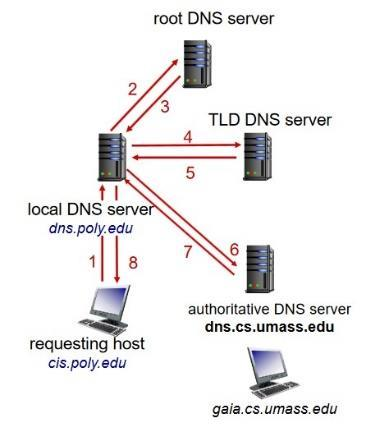
\includegraphics[width = 0.70\textwidth]{./chapter6/DNS_server.jpg}
    \caption{DNS name resolution with iterated query}
    \label{fig:DNS-server}
\end{figure}

